%% report for Natural Gas forward curve simulation

\documentclass[12pt]{article}

\usepackage{graphics,amsmath,pstricks, graphicx}
%\usepackage{hyperref}
%\usepackage[authoryear,round]{natbib}
\usepackage{multicol, multirow}

\textwidth=6.5in
\textheight=8.5in
%\parskip=.3cm
\oddsidemargin=.1in
\evensidemargin=.1in
\headheight=-.5in
\footskip=.7in

\newcommand{\scscst}{\scriptscriptstyle}
\newcommand{\scst}{\scriptstyle}
\newcommand{\Rfunction}[1]{{\texttt{#1}}}
\newcommand{\Robject}[1]{{\texttt{#1}}}
%\newcommand{\code}[1]{{\textit{#1}}}
\newcommand{\code}[1]{{\tt #1}}
\renewcommand{\baselinestretch}{1.2}


\begin{document}
\title{Forward price simulation}
\author{Hao Wu and Adrian Dragulescu}
\maketitle

\section{Background}
Long term price simulation is useful in many aspects.
Simulated forward prices can be used in calculation of 
long term Value at Risk (VaR), potential exposure (PE), 
optimal asset allocation, etc. 

In this project we simulated forward curves for all 
commodity futures contracts in portfolio. 
The simulation is done solely from the finance aspect, ie.,
forward price is simulated based on historical prices. 
We assumed the log prices follow OU  processes
and did simulation from there. 
Because of the strong correlation among curves, 
all curves should be simulated correlatedly. 
Given the scale of the data (30,000+ curves)
it's computationally infeasible to simulate all the data
together. Principal component analysis (PCA) 
was applied to reduce the dimension of the data. 
Futhermore, we built a hierarchy among the curves
so that the simulation can be done sequentially. 
Simulation results look good and the performance
is acceptable.

%% data section
\input data.tex

%%%%%%%%%%%%%%%%%%%%%%%%%%%%%%%%%%%%%%%%%%%%
%% method section
%%%%%%%%%%%%%%%%%%%%%%%%%%%%%%%%%%%%%%%%%%%%
\newpage
\section{Method}

This section will give some technical details for the methods
used in this project. 

\subsection{Orthogonalization and dimension reduction}

There are over 600 curves in portfolio, each one has contracts
for 30 to 120 future months. So totally there are over 30,000
curve-month combinations. As illustrated in previous section,
in each market there are strong correlations 
among curve-months in two direction:
for each curve the prices for all contract months are highly
correlated. Also for each contract month, all curves are correlated.
So ideally all curve-months should be simulated together.
That requires to handle a 30,000 by 30,000 correlation matrix,
which is not feasible computationally. 

Principal component analysis (PCA) is a widely used technique 
in data dimension reduction. It extracts common features from 
correlated data (usually of high dimension) and summarize them
by a few independent data sets called Principal component (PC). 
The dimension can be greatly reduced without lossing much 
information. Probably more important than dimension reduction
in this problem is that
the resulting PCs are independent so that we can break the 
correlations at one direction and do simulation on each group of PCs
separately. 

More specifically, for each curve we applied PCA for its log 
historical price of all contract months and kept the first $K$ 
PCs. Doing so broke the correlations among 
contract months. The correlation among curves were posessed 
in the PCs now, e.g., PC1's for all curves are highly correlated,
so are the PC2's and so on. PC's are orthogonal so 
simulation can be done for each PC independently.
 
To make it formal, let column vector 
$X^c_{t_m}=[x^c_{t_m}(1), x^c_{t_m}(2), \ldots, x^c_{t_m}(T)]^T$, where
$x^c_{t_m}(t)$ denotes the log price at (historical) time
$t$ of future contract with delivery at month $t_m$ for curve $c$,
with $c=1, \ldots, C$, $m=1, \ldots, M$ and $t=1, \ldots, T$. 
The correlations among $X^c_{t_m}$ are in two directions:
\[cov([X^c_{t_1},X^c_{t_2}, \ldots, X^c_{t_M}])=\Sigma^c \mbox{ for }\forall c
\mbox{, and } 
cov([X^1_{t_m}, X^2_{t_m},\ldots, X^C_{t_m}])=\Omega_m \mbox{ for } \forall m. \]
We can do PCA at either direction but we 
have observed that the correlations
among contract months are higher and probably more consistent. 
So it makes more sense to do PCA for each curve. For commodity $c$,
let $\mathbf{X^c}=[X^c_{t_1},X^c_{t_2}, \ldots, X^c_{t_M}]$ be a 
$T$ by $M$ matrix, we can find a rotation matrix $W^c$ of
dimension $M$ by $K$ and let $\mathbf{Y}^c=\mathbf{X}^cW^c$. 
$\mathbf{Y}^c$ is a $T$ by $K$ matrix with independent columns, 
Columns of $\mathbf{Y}^c$ are first $K$ PCs for commodity $c$. 
Let $Y_k^c$, $k=1,\ldots, K$ be columns of $\mathbf{Y}^c$, 
we now have 
\[cov([Y^c_1,Y^c_2, \ldots, Y^c_K])=\Lambda^c,\forall c,
\mbox{ and } cov([Y^1_k,Y^2_k, \ldots, Y^C_k])=\Omega_k^*, \forall k. \]
$\Lambda^c$ are diagonal matrices so PCA transformed the 
correlated ``month'' domain to independent ``PC'' domain. 
Correlation among curves are possessed in $\Omega_k^*$, 
which can be estimated from data. 
In simulation, for each $k$ in $1, \ldots, K$, 
we can independently genearte forward $k^{th}$ PC
(correlatedly among curves) then transform them 
back to get the forward price in original scale.

Due to the great similarities among curves, the first 
a few PCs usually can explain most of the variances. 
Below table shows the percentage of variance explained
by the first 10 PCs for a PWY peak curve. 
One can see that cumulatively the first 5 PCs explains
almost 99\% of the total variances. 
\begin{table}[ht]
\begin{center}
\begin{tabular}{rrrrrr}
  \hline
 & PC 1 & PC 2 & PC 3 & PC 4 & PC 5 \\
  \hline
\% var explained & 0.7962 & 0.1240 & 0.0424 & 0.0168 & 0.0083 \\
Cumulative \% var explained & 0.7962 & 0.9202 & 0.9625 & 0.9794 & 0.9877 \\
\hline \hline
 & PC 6 & PC 7 & PC 8 & PC 9 & PC 10 \\
\hline
\% var explained & 0.0032 & 0.0018 & 0.0012 & 0.0010 & 0.0007 \\
 Cumulative \% var explained & 0.9909 & 0.9928 & 0.9939 & 0.9949 & 0.9956 \\
   \hline
\end{tabular}
\end{center}
\end{table}

Figure \ref{pc-pwy} shows the plot for the first 10 PCs.
The scales of the curves dropped quickly.
\begin{figure}[htbp]
\centering
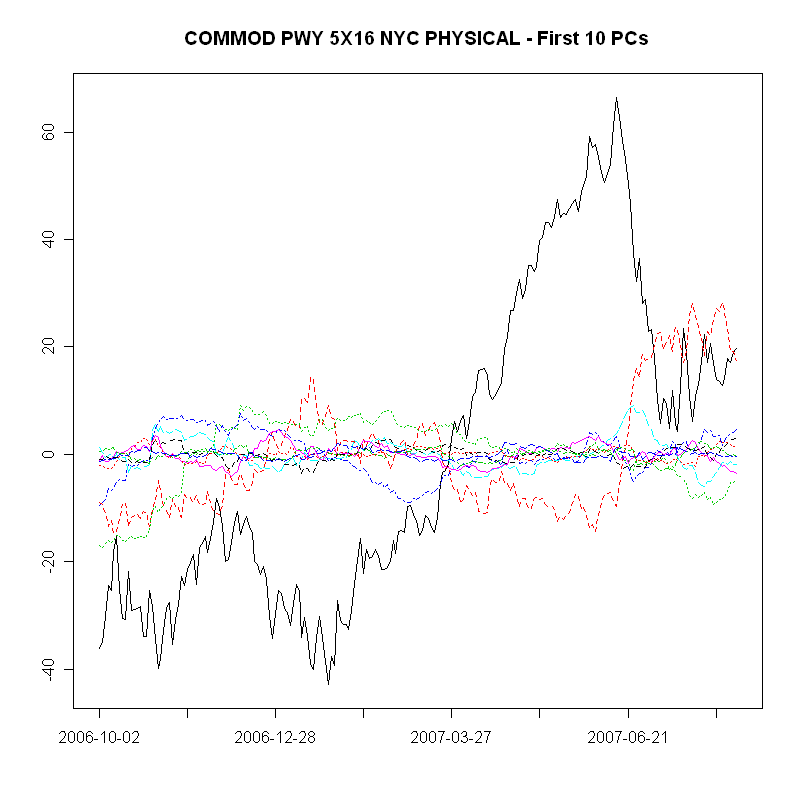
\includegraphics[width=3in, height=3in]{figures/pc-pwy-peak.png}
\caption{First 10 PCs for a PWY peak curve}
\label{pc-pwy}
\end{figure}

\subsection{Curve pedigree}

After breaking the correlation among months by PCA, it seems we are ready 
to simulate. But for each PC there are still over 600 curves.
A 600 by 600 covariance matrix is manageable but inefficient.
More importantly, in the future if we want to adopt more complicated 
methods such as econometrics model, it will be difficult to implement.
So we are looking to further reduce the dimensionality of the problem.
From Data section we can see curves are more similar when their
markets are physically closer. So it's a natural thinking to 
divide the curves into groups by market. Based on these ideas
we built a dependency structure for curves based on 
their commodity type and location. 

We first pick one commodity reference curve for each type of fuels
(NG, COL, FCO, WTI). These four reference curves consists of the
top level of the pedigree. Under that
for natural gas, we divide the North America market into 17 
regions. Each region has a regional reference curve. 
These regional reference NG curves are children of the 
NG commodity reference curve. The rest of the NG curves
are children of their regional reference curve respectively.
For COL, FCO and WTI, we didn't divide the market by region 
at this time so all of the curves are direct 
children of their commodity reference. It will be easy to
add another layer for regions for those commodity 
in the future.  

There are about 20 electricity markets by location. 
A market can have as many as 400 curves (such as PWY). 
From Data section we see all these curves can be roughly 
put into two groups, peak and offpeak. So we pick 
two reference curves in each electricity market,
one for peak and one for offpeak.
We set the parents of these electricity market reference
curves to be three types of fuels: COL, WTI and its nearby
NG regioanl refernce curves. For example the parents 
for PWY reference curves are WTI EXCHANGE, COL NYMEX PHYSICAL
and  NG TRAZN6 NY PHYSICAL. It is possible that
some parents are not correlated with the children curve.
So in that sense the parents we assigned are just ``potential
parents''. A model selection procedure (discussed in later section)
will be used to pick the real parents.

We didn't put any structure on the rest of the commodities 
(freight, emission, etc.) at this time. It would be easy
to assign dependency in the future. 

An illustration of the curve pedigree is shown in Figure 
\ref{peidgree}.
\begin{figure}[htbp]
\centering
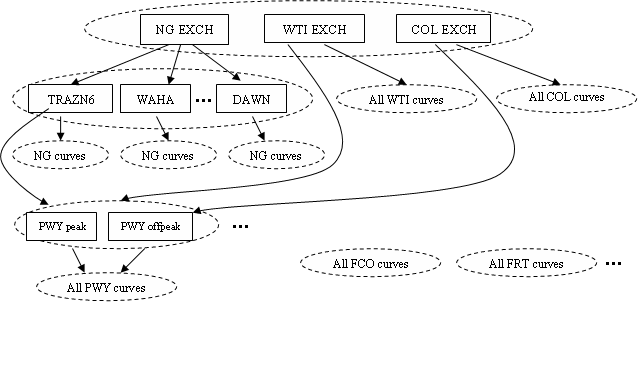
\includegraphics[width=3in, height=2in]{figures/pedigree.png}
\caption{Curve pedigree}
\label{pedigree}
\end{figure}

The curve pedigree is saved as a flat table in an Excel
file, each curve in a row, with around 2400 rows in total.

Now we can do simulations based on the curve pedigree.
We first simulated parents curves then simulate the children
curves conditional on parent curves. 

\subsection{Simulation of parent curves}

Parent curves are defined as 
those without a parent. They don't have to have children. 
For example all CO2 curves are deemed as parent curves
because we didn't assign any parent for them. Parent curves
are simulated in groups in order to keep the correlations
among them. Four commodity refernce curves for
fuels are in the same group. In each of the 
``other markets'', all curves are in the same group. 

We made a critical assumption here that each commodity price 
follows a OU process. With the consideration
of correlations, all curves in the same group 
will  follow correlated 
OU processes. To make it formal, assume
the log price for commodity $c$, contract month $t_m$
follows:
\[dX_{t_m}^c(t) = -\gamma_{t_m}^c \{X_{t_m}^c(t)-\theta_{t_m}^c\}dt 
+ \sigma_{t_m}^c dW_{t_m}^c(t) \mbox{, }  m=1, \ldots, M
\mbox{, } c=1, \ldots, C \]
The Wiener processes $W_{t_m}^c(t)$ for $\forall m, c$
are correlated.

Prior to this step, 
we had applied PCA on log historical prices and broke the correlation
among contract months. Since the PCs are linear transformation of 
log prices, they
will follow OU processes too.
The PCs follow: 
\[dY_{k}^c(t) = -\gamma_{k}^{*c} (Y_{k}^c(t)-\theta_{k}^{*c})dt 
+ \sigma_{k}^{*c} dW_{k}^{*c}(t)\mbox{, }  k=1, \ldots, K
\mbox{, } c=1, \ldots, C \] 

PCA ensures that there are no correlation among 
different PCs for the same commodity, ie, 
$cor(W_{i}^{*c}(t),W_{j}^{*c}(t))=0 \mbox{ for } \forall i\ne j$.
But for the $k^{th}$ PC of all curves, the Wiener processes 
$W_{k}^{*c}(t), c=1,\ldots,C$
are still highly correlated. I will call the same PC (e.g., PC1) for 
all curves ``PC group'' thereafter.
It is worth to mention that there could be correlations
for different PCs between different commodity, ie,
$cor(W_{i}^{*c_1}(t), W_{j}^{*c_2}(t))>0 \mbox{ for some } i\ne j$.
There is no theoretical result to justify the 
indepdendence among them. 
But in practice I found very little correlation, 
mainly because of the strong correlation within each 
PC group. If, say, PC1 and PC2 are independent for commodity 1,
and PC1's for commodity 1 and 2 are very similar.
It is safe to claim that PC1 of commodity 2 and PC2 of 
commodity 1 would be (almost) independent. 

To simulate forward prices, we only need to simulate
each PC group independently, then transform them back.
Within each PC group, all the curves (PC) are still correlated.
In order to simulate correlated OU processes,
we did another round of PCA (PCA on PCs) to orthogonalize them. 
The results (PCs of the PCs) are independent OU processes
and can be simulated easily. 

To summarize, the steps for simulating parents curves are:
\begin{enumerate}
\item Do PCA on each curve to break the 
correlation among contract months, 
\item Iterate following substeps for all PC groups 
to simulate forward PCs correlatedly:
\begin{enumerate}
\item Do PCA on the PCs in the same group to break the correlation among curves. 
This gives independent OU processes. 
\item For each process from previous step, estimate OU parameters
and simulate forward curves.
\item Transform back to get forward PCs for each PC group.
\end{enumerate}
\item Gather the forward PCs for all PC groups then transform 
back to get the forward log prices.
\end{enumerate} 

One VERY important thing is that sometimes the price didn't 
follow OU process. For example is the prices 
kept going up  for all historical days, 
the estimated $\gamma$ will be negative, which means 
there is greater force to push price to continue go up when 
it is further away from the long term mean ($\theta$).
At this time what I did was to make $\gamma$ 
a very small positive number ($10^{-5}$) if the estimated value
is negative. Of course this will produce 
wrong result. However in practice this was only 
found in higher order PCs, which contributes little
in price decomposition. So the simulation result still looks fine.
There are some possible solutions to this.
One is to use longer historical time. Another more
complicated way is to  
decompose the time horizon into ``up'', ``down''
and ``flat'' regions. In each region we can 
remove the longer term trend and fit OU
process on residuals. Anyway this remains an open 
question and is an area for future reseach.


\subsection{Simulation of children curves}

After having all parent curves simulated, we are in place
to simulate the children curves. The children curves
should be generated by group to keep their correlation.
Note that a group of children curves could have different
parents. For example, all electricity market reference
curves are in the same group because we want to correlate
different market, yet their natural gas parents are different. 
We assume the children curves prices follow the parent curves prices.
A multiple linear regression will be the easiest way
to model that dependency. 

Using a set of new notations, let $y(t)$ be log historical prices
for a child curve, and $x_p(t)$ be log historical prices
for its $p^{th}$ parent curve, $p=1, 2, \ldots, P$. 
The most straightforward idea is to regress the 
children's daily prices on the parents' daily prices, e.g.,
\begin{equation}
y(t)=\beta_0 + \sum_{p=1}^P \beta_p x_p(t) + \epsilon(t). 
\label{model1}
\end{equation}
This gives pretty good fit with $R^2$ above 0.85 for 
most of the curves. However there are some problems.
First is that the regression could be ``spurious'' as
referred by some literature so $R^2$ is not reliable. 
Secondly this model assumes that  the children curve 
track parent curves tightly in a daily basis, which 
isn't necessarily  true. 
The most important problem in practice  is that 
there are strong auto-correlation among the residuals 
$\epsilon(t)$. In simulation we want to generate forward
prices sequentially and we want the regression residuals 
are independent from day to day. Auto-correlated
residuals are undesirable.

We then tried to regress the children log returns
on parents' log returns, e.g.,
\begin{equation}
\Delta y(t)=\beta_0 + \sum_{p=1}^P \beta_p \Delta x_p(t) + \epsilon(t). 
\label{model2}
\end{equation}
This model fits the data poorly with $R^2$ dropped dramatically
to around 0.4 for many curves. The reason is obvious:
the children and parent curves are cointegrated.
Although the prices evolve together, their daily log returns 
could be very different. 

Model \ref{model2} can be rewritten as:
\[ y(t)=\beta_0 + y(t-1) + \sum_{p=1}^P \beta_p \{x_p(t)-x_{p}(t-1)\} + \epsilon(t). \]
It actually regress child's today's price $y(t)$ on 
its previous day's price $y(t-1)$ and parents' today
and previous days' prices $x_p(t)$ and $x_p(t-1)$.
The model impose constraints on the coefficients to
force the coefficient for $y(t-1)$ is 1 and 
the coefficients for $x_p(t)$ and $x_p(t-1)$ are
the same in magnitude but with opposite signs.
We relieved these constraints and came up with the following model:
\begin{equation}
  y(t)=\beta_0 + \beta_1 y(t-1) + 
\sum_{p=1}^P \{\beta_{p1} x_p(t) + \beta_{p2} x_p(t-1) \} + \epsilon(t). 
\label{model3}
\end{equation}
Model \ref{model3} fits the data very well and there're very 
little  auto correlation
left in the residuals.
This model can be related to model \ref{model1} as the following. 
Since there are auto-correlations in $\epsilon(t)$ in \ref{model1}, 
we can regress $\epsilon(t)$ on $\epsilon(t-1)$. The residuals
from that regression has very little auto-correlation left. 
This residual regression is equivalent to model \ref{model3}.

Model \ref{model3}  can also be related to 
Error Correction Model (ECM) developed for modeling cointegrated
processes. From model \ref{model3} if we calculate the difference
between $y(t)$ and $y(t-1)$ we get:
\[\Delta y(t) = \beta_1 \Delta y(t-1) + 
\sum_{p=1}^P \{\beta_{p1} \Delta x_p(t) + \beta_{p2} \Delta x_p(t-1) \} + 
\Delta \epsilon(t). \]
In ECM there's no $\Delta x_p(t)$ term because it assumes 
$y(t)$ and $x(t)$ co-evolved. Since we now have the luxury to
know $x(t)$ beforehand, inclusion of $\Delta x_p(t)$ can
improve the model fitting. Note that from ECM one cannot get 
model \ref{model3}. So our model is more liberal.

In practice, all $x(t)$ and $y(t)$ are PCA scores. They
were centered around 0 so the estimated $\beta_0$
should be 0. Therefore we dropped the intercept from
model \ref{model3} to remove possible numerical error 
and have our final model as:
\begin{equation}
  y(t)=\beta_1 y(t-1) + 
\sum_{p=1}^P \{\beta_{p1} x_p(t) + \beta_{p2} x_p(t-1) \} + \epsilon(t). 
\label{model4}
\end{equation}

Note that the parents we assigned to children curves are just
``candidate parent''. They don't have to be correlated with their
children curves or the correlation could be different for different
contract months.
So we did parent curve selection by regression model selection.
In model \ref{model4} if the effects for $x_p(t)$ and $x_p(t-1)$
are not significant (with p-value bigger than 0.05) parent $p$ 
will be dropped from the model. Doing so gives the most
parsimonious model and remove unnecessary noises. 

Now consider multiple correlated children curves
$y_i(t)$, $i=1, \ldots, C$. 
The correlation among children curves is the combination of 
the correlation among their parents and the correlation 
in the residual effects. The first component was correctly
simulated in parent curve simulation. The second component
needs some attention. 
The correlations in residuals from model \ref{model4} 
underestimates the truth. Because the children curves
are also cointegrated but for computational reason
we didn't take that into account (there's no 
$\Delta y_2(t-1)$ in regression model for $y_1(t)$).
We tried and found that 
using residual correlation from model \ref{model4} 
gives poor result. The correlations in simulated forward prices
are underestimated, from above 0.9 in historical prices
to around 0.7 in forward prices. So we use the correlation
in the historical prices as the correlation for residuals.
This will artificially inflate the correlation but considering
the loss of correlation in dimension reduction, this 
can serve as a compensation. The bad thing is
that it forces the daily residuals for all curves to be
very similar. However since the regression $R^2$ is usually
very high ($\ge 0.95$) this effect is minor. 
Simulation shows very good results

Another aspect need to be mention is that our forward
time steps are not constant. We simulated daily data
for some days then do monthly. Should the residual
$\epsilon(t)$ in model \ref{model4} be from the same
distribution? The answer is yes. $\epsilon(t)$ 
can be (kind of) viewed  as the cointegration 
process of the child and parent curves, so it should be
stationary. Another point is that although we didn't 
impose OU assumption on children curves,
they are almost OU since they follow 
their parents (which are OU) closely.


\input sim-result.tex

\newpage
\section{Conclusion and future works}
In this report we have proposed an algorithm for 
forward prices simulation. Given the large scale of the data
we applied principal component analysis to reduce the dimensions
and orthogonalize the curves. One essential assumption is 
that the prices are following OU processes. 
Parameters for the processes were estimated from 
historical data and forward curves were generated 
using the same parameters. 
A hierarchy for curves were built so that we can first simulate
the parent curves, then simulate the children curves accordingly.
Simulation results make good sense. The correlation structure
and volatilities were well preserved.

The program was imlemented using open source programming
language {\tt R}. Computation was done parrally using
open source software package {\tt Condor}. 

There are many areas can be worked on to improve the simulation.
The major problems include:
\begin{enumerate}
\item How to deal with the cases when the 
assumption of OU process is incorrect.
As discussed before we can either use a longer 
historical time or use Hidden Markov Model (HMM) type
of approach to divide the time period into ``up'', ``down''
and ``flat'' periods. Then the trend can be removed and 
OU assumption can be applied on the residuals.
The transition and emission probabilites
can be estimated empirically and used in forward simulation. 
This might work well for short term but I would guess the long term
simulation results will be similar because the trend will cancel
in long term. Also this will introduce much more computations. 
\item Regression models of children curve on parent curves. 
Currently a linear model is implemented to characterize the dependency
but we could choose a different set of basis to capture
the possible nonlinearility in the data. 
\item Instead of using PCA to do dimension reduction, 
one can use nonlinear dimension reduction method,
such as Locally Linear Embedding (LLE) . 
As described by Chen {\it et al.} the nonlinearility
in electricity curves can be well captured by a few (like 3)
intrinsic component, instead of many (currently 10) PCs. 
However according to what I observed, there are
the nonlinearility is not obvious even in electricity curves.
As a result the first 5 PCs can explain over 95\% of
the total variance so the gain from using LLE is not great.
Plus the computation of LLE and 
restruction requires many other extra steps, such as finding nearest 
neighbors, constrainted least square, etc., so the overall
computation might be even more. It seems to be that some simplified version
of  LLE is possibe and promising. Maybe we 
can do one round of LLE on all curve/month combinations 
instead of two rounds of PCA and reduce some computation.
\item In the simulation we assume the volatilities didn't
change along with time. From what we have observed in
the data that is not true sometimes, especially in the 
electricity curves. There are several ways to model the volatility
as a function of time to maturity. ARCH/GARCH type of model
is an obvious choice. Or we can put a functional form 
on the volatility and estimate the paramters from historial data.
\item Finally we took complicated (and hopefully more 
accurate) approaches by introducing other factors, such as
weather forcast, economy growth, transmission/storeage, etc.
This should be done at the parent curves level. 
\end{enumerate}



\end{document}
